% \subsection{Physical limits with ``fair'' queuing}
% \label{sec:queuing}

% However, this limitation approach does not attempt to utilize data plane performance knowledge (i.e., Interest satisfaction ratio statistics) to discriminate good and malicious Interests.

To address the lack of fairness associated with the naive {\it Token Bucket} algorithm, we modify it to ensure that the Interests forwarded by a router on each interface represent a fair mix of Interests received from neighboring interfaces. For example, in Fig.~\ref{fig:flooding example} router A can ensure that the tokens associated with Interests sent out on interface {\texttt eth2}  are fairly distributed across incoming interfaces \texttt{eth0} and \texttt{eth1}. 
%Due to the expected small volume of Interests, we cannot merely rely on network buffers to perform statistical multiplexing of Interests, as they would almost never be %buffered.
%At the same time, until bag of tokens is not empty, there is no reason to delay Interest forwarding, as we do not known how many and from which interfaces Interests %will arrive in the future.
In order to achieve our goal of ensuring ``fair'' mixing of Interests from all neighboring interfaces, 
%, we implement an additional features to support buffering of Interests, if they cannot be immediately forwarded. 
we extend the Pending Interest Table to support flagging of Interests that cannot be immediately forwarded (see Fig.~\ref{fig:queueing}). To support fair queuing, we implement hierarchical queues for each interface as shown in Fig.~\ref{fig:queueing})\footnote{This mechanism is essentially class based queuing, with classes for each outgoing/incoming interface.} As an alternative to hierarchical queues, one can also use an approach based on virtual time. For details, please see ~\cite{zhang1990virtual}.  We note that unlike normal queuing, Interest queues do not actually store a packet, but merely a bi-directional pointer to the existing PIT entry.
Thus, a PIT entry can be quickly updated when the Interest is actually forwarded; further the element can be quickly removed from the queue when the Interest expires.

%For the buffering part, we can reuse Pending Interest Table, with a small extension to support flagging of the Interests that cannot be forwarded immediately (see example on Fig.~\ref{fig:queueing}). 
%As for the mixing part, we need an additional fair queuing mechanism, which can be implemented in a form of hierarchical queues (on Fig.~\ref{fig:queueing})\footnote{This essentially is a class based queuing, with classes for each outgoing/incoming interface.} or using virtual time approach~\cite{zhang1990virtual}. 

\begin{figure}[htbp]
  \centering
  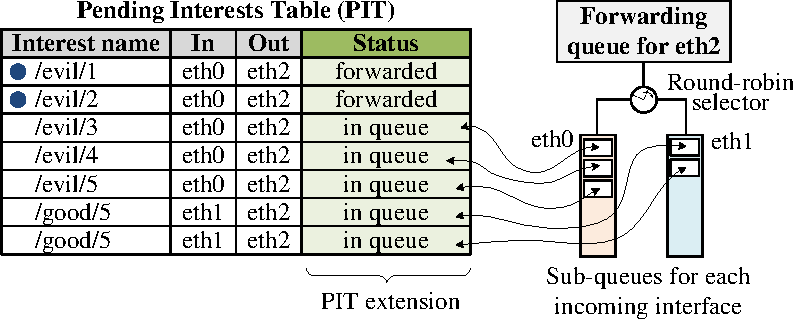
\includegraphics[scale=0.65]{queue}
  \caption{Interest queuing: if tokens are unavailable, the router creates a PIT entry, but instead of forwarding, it enqueues the Interest}
  \label{fig:queueing}
\end{figure}

We present a more formalized description of this algorithm in Pseudocode~\ref{alg:queuing}. We can control the amount of physical resources utilized at a router (such as memory and computation power) by setting appropriate queue sizes. It is also important to set apprpriate value for how long an Interest can be enqueued. If an Interest is enqueued for a long time, by the time it is dequeued and appropriately forwarded, the resulting Data packet might not be valid due to state expiration at previous downstream routers. We believe that implementing additional mechanisms on each pair of communicating routers to keep the Interests from getting stale would mitigate this issue, though the details are beyond the scope of this paper.
{\it Priya:  We need to  touch upon the Interest freshness issue in the NDN overview section; else we should get rid of this bit.}

%It should be noted that enqueued Interests should not be kept in the queue for a prolonged period of time.
%Otherwise, by the time the Interests reaches the Data, the state could have been long expired downstream, effectively making such an Interest useless.
%Additional mechanisms of pair-wise agreements between NDN routers and periodic Interest refresh can solve this particular problem, but it is out of the scope of the present paper.

%The algorithm extends the base Physical limits algorithm by enabling queuing when the bag of tokens is empty (lines 7--10), as well as by triggering an action (lines 16--21), when a token becomes available and enqueued Interest can be finally forwarded.
%At the same time, the algorithm limits number of Interests allowed in a queue, constraining memory usage increase by at most a constant factor, compared to the base Physical limits algorithm (i.e., memory attack on routers are still unfeasible). 


\floatname{algorithm}{Pseudocode}

%%%%%%%%%%%%%%%%%%%%%%%%%%%%%%
%%%%%%%%%%%%%%%%%%%%%%%%%%%%%%
%%%%%%%%%%%%%%%%%%%%%%%%%%%%%%

\begin{algorithm}[h]
\footnotesize
\caption{\small Physical limits with per-interface fairness}
\label{alg:queuing}
\begin{algorithmic}[1]
\State{} \Comment{Same initialization, InData and Timeout functions as in Physical Limits algorithm}

\vspace{0.2cm}

\Function{OutInterest}{Interest \textbf{i}, InInterface \textbf{if}, OutInterface \textbf{of}}
    \If{$L_{of} - O_{of} > 0$} \Comment{\textbf{of} is under physical limits}
        \State $O_{of} \leftarrow O_{of} + 1$  \Comment{``Borrow'' token}
        \State add \textbf{of} to PIT entry and forward \textbf{i} to \textbf{of}
    \Else
        \State Queue $q \leftarrow of$.GetSubQueue($if$)
        \If{$Size(q) < L_{of}$}
           \State $q$.PushInterest($i$)
           \State add \textbf{of} to PIT entry, and link PIT entry with the queue
        \Else
           \State drop Interest
        \EndIf
    \EndIf
\EndFunction

\vspace{0.2cm}
\State{} \Comment{\textit{Whenever $L_{of} - O_{of}$ becomes larger than zero}}
\Function{TokenBecomesAvailable}{}
    \State Queue $q \leftarrow$ $of$.GetRoundRobinSubQueue 
    \State $i \leftarrow$ $q$.PopInterest
    \State update PIT entry and Forward($i$, $of$)
\EndFunction
\end{algorithmic}
\end{algorithm}


As we show in Section~\ref{sec:evaluation}, fair queueing provides partial relief from the Interest flooding attack, allowing legitimate users to successfully fetch Data for 15--20\% of the expressed Interests (compared to 0-10\% without fair queueing). While this algorithm might be reasonable for ensuring fairness in an NDN network, it is completely ineffective in protecting legitimate users from malicious attackers. Malicious attackers are able to successfully thwart access to content for legitimate users by sending a relatively modest volume of Interests.


%At the same time, the Physical limits with or without fair queueing allows attackers to send a relatively small volume of Interests in order to significantly impact service for the legitimate users.
%Therefore, to successfully solve the problem, we need a fundamentally different, more intelligent approach, allowing localization of the attack traffic as close as possible to the attack origin.

%%% Local Variables: 
%%% mode: latex
%%% TeX-master: "../paper"
%%% End: 
